\chapter[Modèle de Riesz]{Étude théorique du modèle de Riesz} % signal monogénique ?
\label{chap:chapitre1}

Dans le but de synthétiser du contenu avec de la structure irrégulière, une approche locale est adoptée. Ce travail utilise le modèle du signal monogène~\cite{felsberg_monogenic_2001}, qui permet d'extraire l'énergie locale, en s'appuyant sur la transformée de Riesz. Le signal monogène est ensuite mis en application dans un cadre multi-résolutionnel, en utilisant une pyramide de Riesz~\cite{wadhwa_riesz_2014} pour calculer la congruence de phases.

\section{Signal monogène}

Le signal monogène est un outil du domaine du traitement du signal introduit par Felsberg et Sommer~\cite{felsberg_monogenic_2001}. Le signal monogène est utilisé pour des tâches d'analyse d'image ou de vision par ordinateur, comme la détection de caractéristiques. La revue de la méthode par Bridge~\cite{bridge_introduction_2018} est une introduction simple et compréhensive aux principes théoriques du signal monogène. Le travail de Bridge est repris dans cette partie, ainsi que ses notations et son discours, afin de prodiguer une compréhension du modèle.

\subsection{Une dimension, signal analytique}

\subsubsection{Construction du signal analytique}

Pour comprendre l'utilité du signal monogène, il faut expliquer le fonctionnement du signal analytique. Le signal monogène est ensuite défini comme l'extension du signal analytique aux signaux de dimension arbitraire. Le signal analytique est une méthode de représentation d'un signal 1D à valeurs réelles, qui facilite la manipulation et l'extraction de certaines informations du signal original. Le constat qui donne lieu à cette représentation est que pour un signal à valeurs réelles, les fréquences négatives sont superflues pour sa représentation de Fourier. En effet, la transformée de Fourier $F(\omega)$ d'un signal à valeurs réelles $f(t)$ présente une symétrie hermitienne :

\begin{equation}
    F(-\omega) = \overline{F(\omega)}
\end{equation}

avec $\overline{\cdot}$ l'opérateur de conjugaison complexe. Les fréquences négatives, non-nécessaires, peuvent donc être mises de côté sans perte d'information. Un nouveau signal est construit en n'utilisant que les fréquences positives de $f(t)$. Le signal $F_{\alpha}$ est d'abord exprimé dans le domaine de Fourier :

\begin{equation}
    F_{\alpha}(\omega) = \left\{
    \begin{array}{ll}
        2F(\omega), & \omega > 0 \\
        0, & \omega < 0 \\
        F(0), & \omega = 0,
    \end{array}
    \right.
\end{equation}

où l'amplitude des composantes de fréquences positives est doublée, par soucis de conservation d'énergie. Avec cette formulation, toute l'information du signal original est conservée. Cette nouvelle forme permet en plus de faire des manipulations précédemment impossibles, qui permettent de mieux comprendre le signal.

\begin{figure}[h]
    %\noindent
    \hspace{-12pt}
    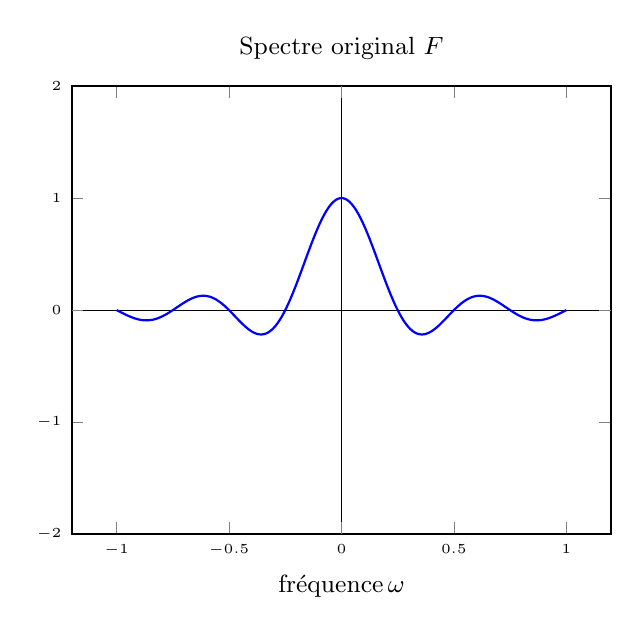
\begin{tikzpicture}
    \begin{axis}[
        title={Spectre original $F$},
        title style={font=\small},
        axis lines=box,
        style=thick,
        xlabel=\(\textnormal{fréquence}\, \omega\),
        xtick={-1, -0.5, 0.5, 1},
        ytick={-2, -1, 1, 2},
        extra x ticks=0,
        extra y ticks=0,
        extra x tick style={grid=major, grid style={black}},
        extra y tick style={grid=major, grid style={black}},
        tick label style={font=\tiny},
        label style={font=\small},
        ymin=-2, 
        ymax=2,
        ]
    \addplot[
        color=blue,
        domain=-1:1,
        samples=200
        ]
    {sin(360*x*2)/ (2*pi*x*2)};
    \end{axis}
    \end{tikzpicture}
    %\hskip 6pt
    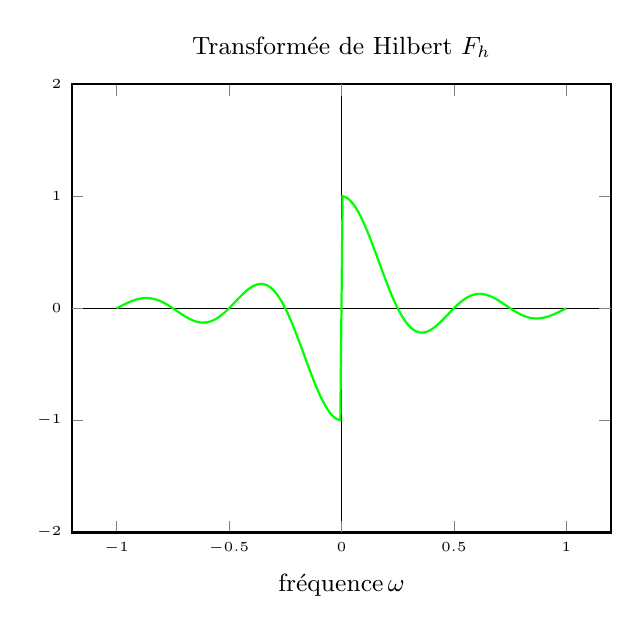
\begin{tikzpicture}
    \begin{axis}[
        title={Transformée de Hilbert $F_h$},
        title style={font=\small},
        axis lines=box,
        style=thick,
        xlabel=\(\textnormal{fréquence}\, \omega\),
        xtick={-1, -0.5, 0.5, 1},
        ytick={-2, -1, 1, 2},
        extra x ticks=0,
        extra y ticks=0,
        extra x tick style={grid=major, grid style={black}},
        extra y tick style={grid=major, grid style={black}},
        tick label style={font=\tiny},
        label style={font=\small},
        ymin=-2, 
        ymax=2,
        ]
    \addplot[
        color=green,
        domain=-1:1,
        samples=200
        ]
    {sign(x)*sin(360*x*2)/ (2*pi*x*2)};
    \end{axis}
    \end{tikzpicture}
    %\hskip 6pt
    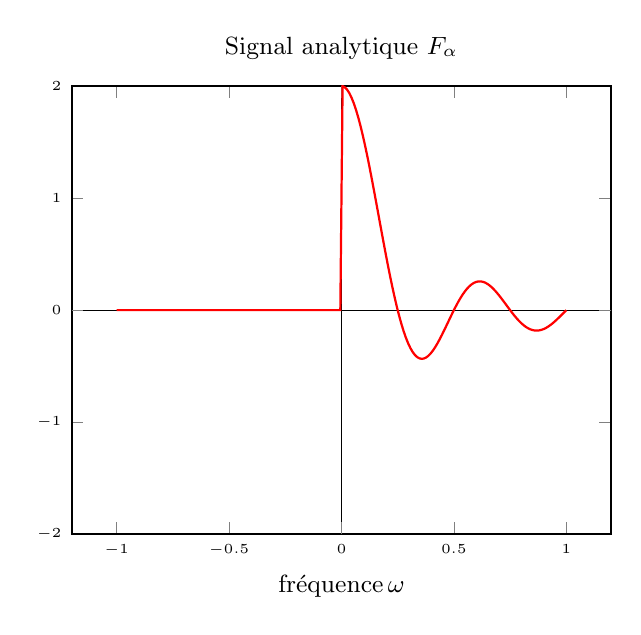
\begin{tikzpicture}
    \begin{axis}[
        title={Signal analytique $F_{\alpha}$},
        title style={font=\small},
        axis lines=box,
        style=thick,
        xlabel=\(\textnormal{fréquence}\, \omega\),
        xtick={-1, -0.5, 0.5, 1},
        ytick={-2, -1, 1, 2},
        extra x ticks=0,
        extra y ticks=0,
        extra x tick style={grid=major, grid style={black}},
        extra y tick style={grid=major, grid style={black}},
        tick label style={font=\tiny},
        label style={font=\small},
        ymin=-2, 
        ymax=2,
        ]
    \addplot[
        color=red,
        domain=-1:1,
        samples=200
        ]
    {(1+sign(x))*sin(360*x*2)/ (2*pi*x*2)};
    \end{axis}
    \end{tikzpicture}

    \caption[Signal analytique pour un signal simple]{Création du signal analytique dans le domaine fréquentiel (seule la partie réelle est montrée). Le signal original réel (gauche), qui présente une symétrie hermitienne, est ajouté à sa transformée de Hilbert (milieu), lui impair, pour former le signal analytique (droite), dépourvu de fréquence négative.}
    \label{fig:complex-analytic-representation}
\end{figure}

La suppression des composantes de fréquences peut être vue comme l'ajout d'un certain signal impair au signal de base.

\begin{equation} \label{eq:2.1}
    F_{\alpha}(\omega) = F(\omega) + F_h(\omega)
\end{equation}

La formation du signal analytique est montrée dans la figure~\ref{fig:complex-analytic-representation}. Dans l'équation~\ref{eq:2.1}, $F_h(\omega)$ est la « version impaire » du signal $F(\omega)$ :

\begin{equation}
    F_h(\omega) = \left\{
    \begin{array}{ll}
        F(\omega), & \omega > 0 \\
        -F(\omega), & \omega < 0 \\
        0, & \omega = 0,
    \end{array}
    \right.
\end{equation}

qui se reformule à l'aide de la fonction signe :

\begin{equation}
    F_h(\omega) = \sgn(\omega)\cdot F(\omega).
    \label{eq:2.5}
\end{equation}

L'expression de la fonction signe est la suivante :

\begin{equation}
    \sgn(x) = \left\{
    \begin{array}{ll}
        1, & x > 0 \\
        -1, & x < 0 \\
        0, & x = 0.
    \end{array}
    \right.
\end{equation}

L'équation~\ref{eq:2.1} est ainsi ré-écrite comme suit :

\begin{equation}
    F_{\alpha}(\omega) = (1+\sgn(\omega))F(\omega)
\end{equation}

\begin{figure}[h]
    %\noindent
    %\hspace{-10pt}
    \centering
    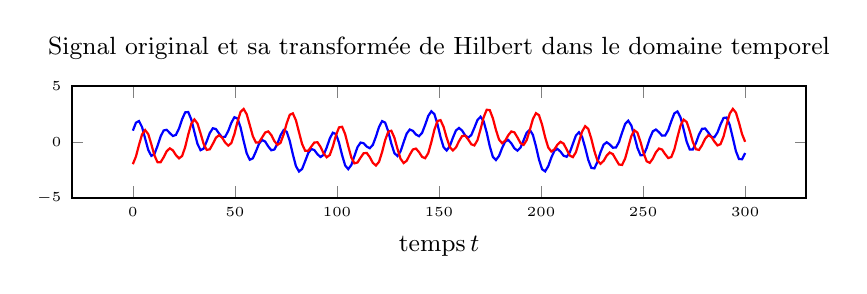
\begin{tikzpicture}
    \begin{axis}[
        title={Signal original et sa transformée de Hilbert dans le domaine temporel},
        title style={font=\small},
        axis lines=box,
        width=0.9\textwidth,
        height=3cm,
        style=thick,
        xlabel=\(\textnormal{temps}\, t\),
        xtick={0, 50, 100, 150, 200, 250, 300},
        ytick={-5, 0, 5},
        tick label style={font=\tiny},
        label style={font=\small},
        ymin=-5, 
        ymax=5,
        ]
    \addplot[
        color=blue,
        domain=0:300,
        samples=200
        ]
    {sin(3*x)+cos(15*x)+sin(30*x)};
    \addplot[
        color=red,
        domain=0:300,
        samples=200
        ]
    {-cos(3*x)+sin(15*x)-cos(30*x)};
    \end{axis}
    \end{tikzpicture}

    \caption[Signal analytique pour un signal complexe]{Exemple de représentation analytique. Le signal original réel (en bleu) et sa transformée de Hilbert imaginaire pure (en rouge).}
    \label{fig:analytic-representation}
\end{figure}

Le signal $F_{\alpha}$ créé est la somme dans le domaine fréquentiel de $F$, signal original pair, et de $F_h$, signal impair. Dans le domaine temporel, les représentations de $F$
et $F_h$ sont purement réelle et purement imaginaire respectivement. La représentation dans le domaine temporel de $F_h$ est nommée $f_h$. Dans le domaine temporel, $f_{\alpha}$ est donc un signal complexe sans composantes de fréquences négatives. $f_\alpha$ est un signal analytique et est appelé la \og représentation analytique \fg de $f$ :

\begin{equation}
    f_{\alpha}(t) = \underbrace{f(t)}_\text{réel pur} + \underbrace{f_h(t)}_\text{imaginaire pur}.
\end{equation}

Le signal ajouté pour annuler les fréquences $F_h$ est par ailleurs un objet connu : c'est la transformée de Hilbert de $F$. Sa représentation, bien que très simple dans le domaine fréquentiel, est difficile à obtenir et manipuler dans le domaine temporel :

\begin{equation}
    f_h(t) = i \cdot \textnormal{p.v.} \int_{-\infty}^{\infty} \frac{f(t)}{\pi(t-\tau)} \,d\tau,
\end{equation}

où p.v. est la valeur principale de Cauchy. Cette intégrale représente la convolution avec la distribution $\frac 1{\pi t}$. L'intégrale est impropre à cause de la singularité en $t=\tau$. La valeur principale est nécessaire pour définir correctement cet objet. Dû à la complexité de l'intégrale, l'expression fréquentielle de la transformée de Hilbert est utilisée à la place :

\begin{align*}
    &\hil(F) = F_h = \sgn\cdot F \\
\end{align*}


\subsubsection{Amplitude et phase locales}

Pour comprendre l'intérêt du signal analytique, l'exemple d'une fonction sinusoïdale, d'amplitude $A$ et de fréquence $\omega_0$ fixées est présenté :

\begin{equation}
    f(t) = A\sin(\omega_0t).
\end{equation}

La transformée de Hilbert de $f$ est calculée en utilisant les relations présentées précédemment, ce qui donne la représentation analytique du signal :

\begin{align}
    f_h(t) &= iA\cos(\omega_0t) \\
    f_{\alpha}(t) &= f(t) + f_h(t) \\
    &= A\sin(\omega_0t)+iA\cos(\omega_0t) \\
    &= Ae^{i\omega_0t}.
\end{align}

Pour une sinusoïde, la transformée de Hilbert est un simple déphasage de $-\frac{\pi}2$ du signal original. Or la théorie de Fourier indique que n'importe quel signal générique peut être décomposé comme une somme de sinusoïdes. La transformée de Hilbert agit donc de la même manière sur tous les signaux : c'est un déphasage de $-\frac{\pi}2$ de chaque composante fréquentielle qui compose le signal. Le signal $f$ et sa transformée de Hilbert $f_h$ sont dits en \og quadrature de phase \fg. Le signal analytique s'exprime comme une exponentielle complexe.

\bigskip

Puisque tout signal est représenté comme la somme d'un réel et d'un imaginaire pur, il est possible d'utiliser une représentation en coordonnées polaires pour exprimer l'exponentielle complexe. L'amplitude et la phase du signal sont alors variables au cours du temps :

\begin{equation}
    f_{\alpha} (t) = A(t)e^{i\phi(t)}.
\end{equation}

avec 

\begin{align}
    A(t) &= \sqrt{f(t)^2 + h_h(t)^2} \\
    \phi(t) &= \arctan\left(\frac{f_h(t)}{f(t)}\right).
\end{align}

Cette représentation introduit le concept d' \og amplitude locale \fg et de \og phase locale \fg (ici temporellement locales). L'amplitude et la phase locales sont deux outils d'analyse particulièrement intéressants pour l'étude approfondie du signal original. L'amplitude locale agit comme une mesure de l'enveloppe du signal. La phase locale agit comme une mesure de la forme du signal. Par exemple, une phase de $0$ indique un extremum, et une phase de $\pm\pi$ indique un passage par zéro. La figure~\ref{fig:local-pha-amp} montre un signal avec son amplitude locale et sa phase locale. À partir uniquement du signal initial, de l'information sur des caractéristiques et sur l'apparence du signal est obtenue.

\begin{figure}[h]

    \centering
    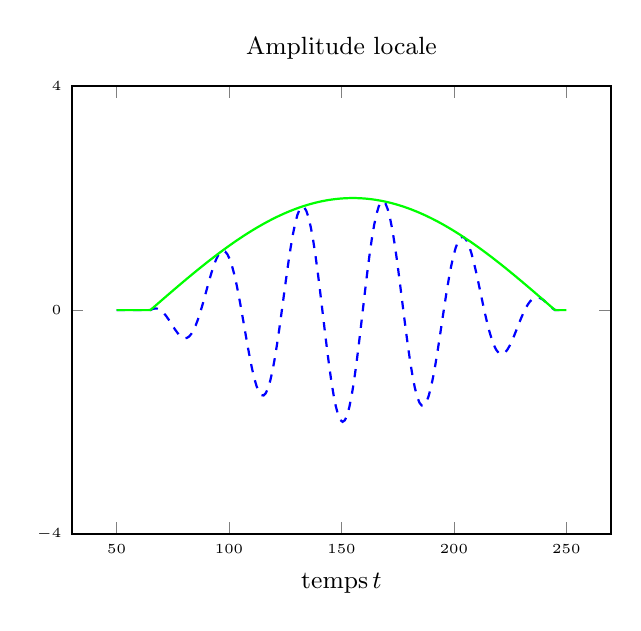
\begin{tikzpicture}
    \begin{axis}[
        title={Amplitude locale},
        title style={font=\small},
        axis lines=box,
        %width=0.9\textwidth,
        %height=3cm,
        style=thick,
        xlabel=\(\textnormal{temps}\, t\),
        xtick={50, 100, 150, 200, 250},
        ytick={-4, 0, 4},
        tick label style={font=\tiny},
        label style={font=\small},
        ymin=-4, 
        ymax=4,
        ]
    \addplot[
        color=blue,
        domain=50:250,
        samples=200,
        style=dashed,
        ]
    {(sign(x-65)-sign(x-245))*sin(10*x+25)*cos(x+25)};
    \addplot[
        color=green,
        domain=50:250,
        samples=200
        ]
    {(sign(x-65)-sign(x-245))*sqrt((0.5*(sin(11*x-40) + sin(9*x-90)))^2 + (sin(10*x+25)*cos(x+25))^2)};
    \end{axis}
    \end{tikzpicture}
    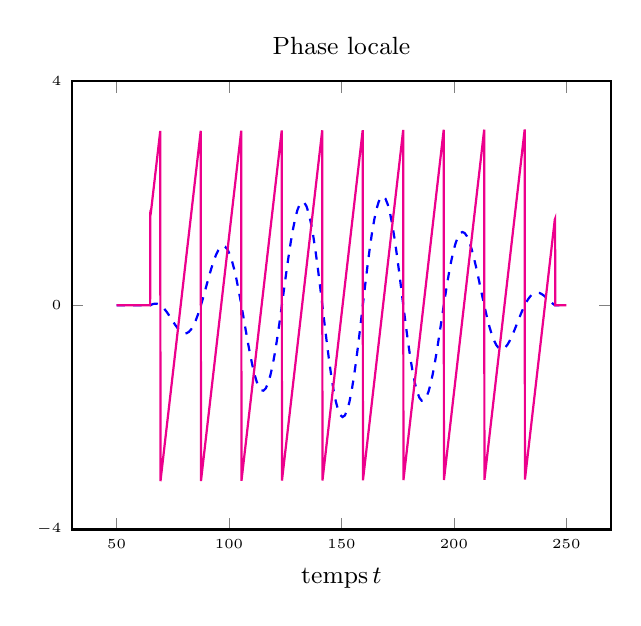
\begin{tikzpicture}
    \begin{axis}[
        title={Phase locale},
        title style={font=\small},
        axis lines=box,
        %width=0.9\textwidth,
        %height=3cm,
        style=thick,
        xlabel=\(\textnormal{temps}\, t\),
        xtick={50, 100, 150, 200, 250},
        ytick={-4, 0, 4},
        tick label style={font=\tiny},
        label style={font=\small},
        ymin=-4, 
        ymax=4,
        ]
    \addplot[
        color=blue,
        domain=50:250,
        samples=200,
        style=dashed,
        ]
    {(sign(x-65)-sign(x-245))*sin(10*x+25)*cos(x+25)};
    \addplot[
        color=magenta,
        domain=50:250,
        samples=2000
        ]
    {(sign(x-65)-sign(x-245))*rad(atan((0.5*(sin(11*x-40) + sin(9*x-90))) / (sin(10*x+25)*cos(x+25))))};
    \end{axis}
    \end{tikzpicture}

    \caption[Informations locales pour un signal simple]{Extraction d'informations locales pour un cosinus modulé par un sinus. L'amplitude locale (gauche) donne l'enveloppe de la sinusoïde, et la phase locale (droite) donne de l'information quant à la position dans le cycle d'oscillation.}
    \label{fig:local-pha-amp}

\end{figure}

\subsubsection{Notion d'échelle}
\label{subsubsec:echelle}

L'exemple donné avec la figure~\ref{fig:local-pha-amp} fonctionne bien car le signal est simple. L'interprétation de l'amplitude et la phase locale est claire et visuelle. Pour un signal plus complexe, plus représentatif des signaux étudiés, l'interprétation des informations locales est moins directe. La figure~\ref{fig:complex-local-pha-amp} affiche les informations locales du signal de la figure~\ref{fig:analytic-representation}, une somme de trois sinusoïdes de fréquences différentes. Les informations locales semblent décorrélées du signal complexe, ou le lien n'est pas directement apparent.

\bigskip

\begin{figure}[h]
    \centering
    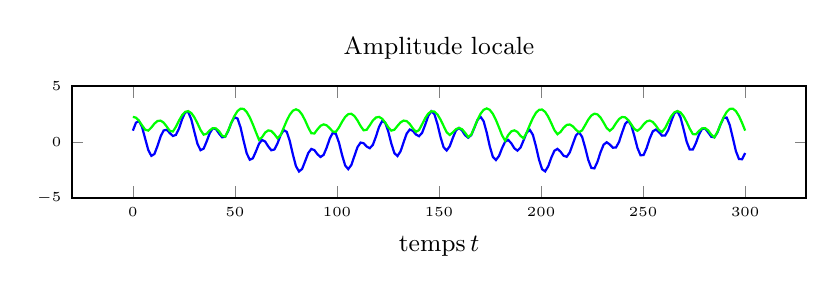
\begin{tikzpicture}
    \begin{axis}[
        title={Amplitude locale},
        title style={font=\small},
        axis lines=box,
        width=0.9\textwidth,
        height=3cm,
        style=thick,
        xlabel=\(\textnormal{temps}\, t\),
        xtick={0, 50, 100, 150, 200, 250, 300},
        ytick={-5, 0, 5},
        tick label style={font=\tiny},
        label style={font=\small},
        ymin=-5, 
        ymax=5,
        ]
    \addplot[
        color=blue,
        domain=0:300,
        samples=200
        ]
    {sin(3*x)+cos(15*x)+sin(30*x)};
    \addplot[
        color=green,
        domain=0:300,
        samples=200
        ]
    {sqrt((sin(3*x)+cos(15*x)+sin(30*x))^2 + (-cos(3*x)+sin(15*x)-cos(30*x))^2)};
    \end{axis}
    \end{tikzpicture}
    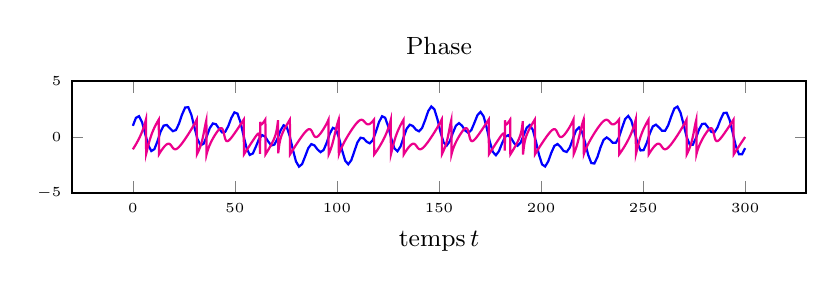
\begin{tikzpicture}
    \begin{axis}[
        title={Phase},
        title style={font=\small},
        axis lines=box,
        width=0.9\textwidth,
        height=3cm,
        style=thick,
        xlabel=\(\textnormal{temps}\, t\),
        xtick={0, 50, 100, 150, 200, 250, 300},
        ytick={-5, 0, 5},
        tick label style={font=\tiny},
        label style={font=\small},
        ymin=-5, 
        ymax=5,
        ]
    \addplot[
        color=blue,
        domain=0:300,
        samples=200
        ]
    {sin(3*x)+cos(15*x)+sin(30*x)};
    \addplot[
        color=magenta,
        domain=0:300,
        samples=3000
        ]
    {rad(atan((-cos(3*x)+sin(15*x)-cos(30*x)) / (sin(3*x)+cos(15*x)+sin(30*x))))};
    \end{axis}
    \end{tikzpicture}    

    \caption[Informations locales pour un signal complexe]{Informations locales pour un signal complexe, somme de plusieurs sinusoïdes. Pour un tel signal, l'interprétation des informations locales est moins directe.}
    \label{fig:complex-local-pha-amp}
\end{figure}

Le problème à l'analyse de ce signal est le fait qu'il existe plusieurs niveaux de structure, comme expliqué dans la section~\ref{subsec:structure}. Les différents niveaux de structure interfèrent et rendent l'interprétation des informations locales impossible à l'échelle macroscopique. Pour extraire de l'information interprétable, il faut sélectionner et faire l'analyse d'un seul niveau de structure, donc d'échelle. Un filtrage est fait pour sélectionner un niveau de structure en particulier et enlever les composantes des niveaux non désirés. Pour filtrer les niveaux de structure, il est possible d'utiliser des filtres passe-bande. Les filtres log-Gabor, utilisés par Bridge, sont un choix commun pour ce genre de pratique. Un filtre log-Gabor permet de sélectionner une bande de fréquence centrée autour d'une fréquence centrale $\omega_0$. Les filtres log-Gabor sont définis dans le domaine fréquentiel et ont une réponse en fréquence de forme gaussienne quand observés en échelle logarithmique :

\begin{equation}
    G(\omega) = \exp\left(-\frac{\log^2(\frac{|\omega|}{\omega_0})}{2\log(\sigma_0)^2}\right).
\end{equation}

Ces filtres sont caractérisés par deux paramètres : la fréquence centrale $\omega_0$ et et la largeur de bande $\sigma_0$. La fréquence centrale contrôle quelle échelle de structure est sélectionnée. La largeur de bande est un paramètre de forme qui contrôle la largeur de la bande de fréquence sélectionnée. Des exemples de filtre log-Gabor sont montrés à la figure~\ref{fig:log-gabor-filters}.

\bigskip

Le filtre log-Gabor est appliqué au signal avant de lui appliquer la transformée de Hilbert et de déterminer sa forme analytique. Le signal filtré offre une représentation locale en fréquence, centrée autour d'une fréquence $\omega_0$ et d'une échelle $\sigma_0$ variable arbitrairement.

\begin{equation}
    F_{\alpha}(\omega) = (1+\sgn(\omega))G(\omega)F(\omega)
\end{equation}

\begin{figure}
    \centering
    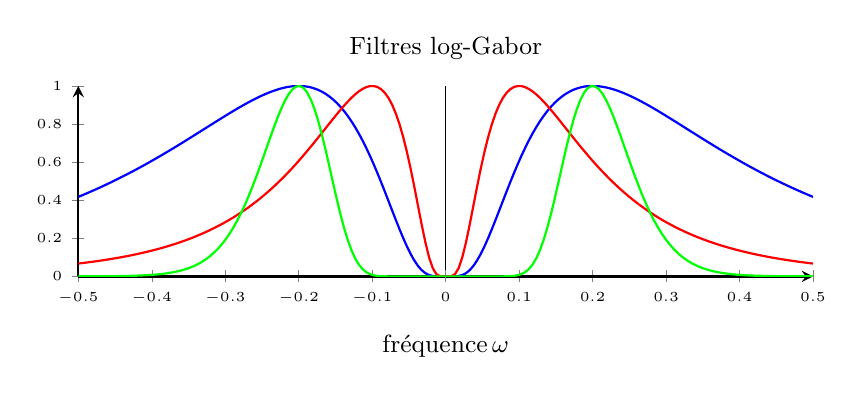
\begin{tikzpicture}
    \begin{axis}[
        title={Filtres log-Gabor},
        title style={font=\small},
        axis lines=left,
        width=0.9\textwidth,
        height=4cm,
        style=thick,
        xlabel=\(\textnormal{fréquence}\, \omega\),
        xtick={-0.5, -0.4, -0.3, -0.2, -0.1, 0.1, 0.2, 0.3, 0.4, 0.5},
        ytick={0, 0.2, 0.4, 0.6, 0.8, 1},
        tick label style={font=\tiny},
        label style={font=\small},
        extra x ticks=0,
        extra x tick style={grid=major, grid style={black}},
        ymin=0,
        ymax=1,
        ]
    \addplot[
        color=blue,
        domain=-0.5:0.5,
        samples=200
        ]
    {exp(-ln(abs(x)/.2)^2 / (2*ln(.5)^2))};
    \addplot[
        color=red,
        domain=-0.5:0.5,
        samples=200
        ]
    {exp(-ln(abs(x)/.1)^2 / (2*ln(.5)^2))};
    \addplot[
        color=green,
        domain=-0.5:0.5,
        samples=200
        ]
    {exp(-ln(abs(x)/.2)^2 / (2*ln(.8)^2))};
    \end{axis}
    \end{tikzpicture}

    \caption[Filtres log-Gabor]{Représentation dans le domaine fréquentiel de filtres log-Gabor de différents paramètres. En rouge, $\omega_0=0.1, \sigma_0 = 0.5$. En bleu, $\omega_0=0.2, \sigma_0 = 0.5$. En vert, $\omega_0=0.2, \sigma_0 = 0.8$.}
    \label{fig:log-gabor-filters}
\end{figure}

Étudier la réponse du signal sur une large gamme de fréquences et d'échelles offre une représentation locale du signal à différentes échelles. La représentation du signal à différentes échelles permet d'extraire de l'information sur les différentes structures du signal. Les informations locales sont présentées dans un graphique appelé \og scalogramme \fg. Le scalogramme montre la réponse d'un signal en fonction du temps et de l'échelle, comme montré à la figure~\ref{fig:scalogram}. Les différents niveaux de structure du signal y sont visibles. Choisir le niveau d'échelle étudié donne un meilleur sens à l'interprétation des informations locales.

\bigskip

Les informations obtenues avec le signal analytique sont différentes de celles obtenues avec la transformée de Fourier. Les informations des deux modèles diffèrent et se complètent. La transformée de Fourier donne de l'information globale sur tout le signal, mais localisée en termes de fréquence. La représentation analytique, elle, donne une information spatialement locale sur le signal, mais sur une bande de fréquences sélectionnée par un filtre passe-bande. Le modèle d'information locale est donc un compromis entre la localisation spatiale et fréquentielle.


\begin{figure}
    \centering
    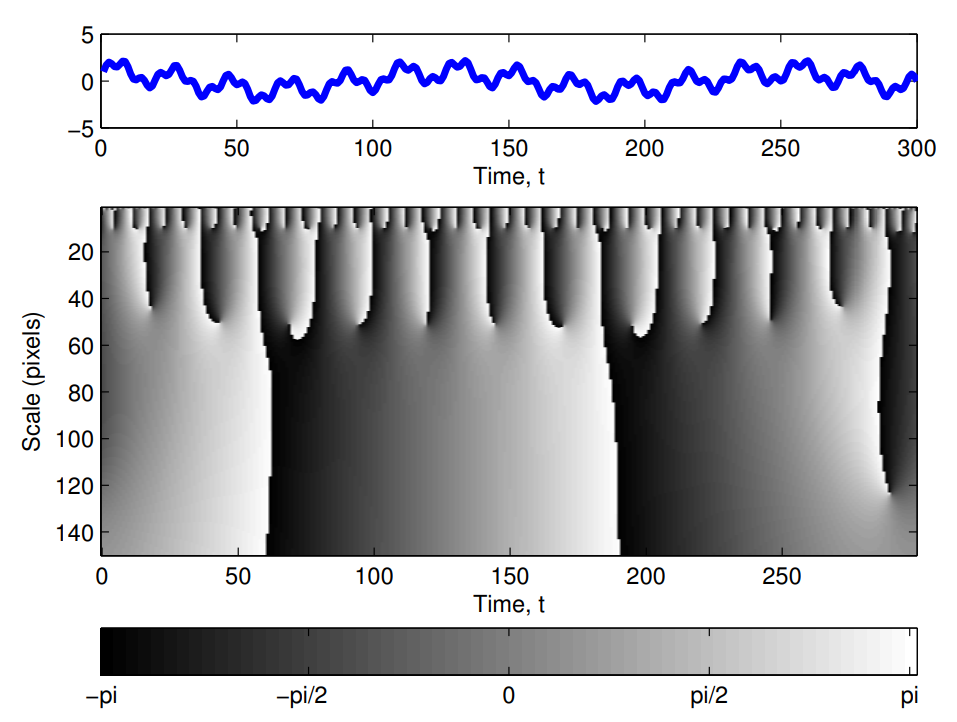
\includegraphics[width=\textwidth]{contenu/resources/images/scalogram}
    \caption[Scalogramme de la phase locale]{Scalogramme de la phase locale pour un signal complexe. La phase locale est représentée en échelle de gris et varie en fonction du temps (en abscisse) et de l'échelle en nombre de pixels (en ordonnée). Diagramme par Bridge~\cite{bridge_introduction_2018}.}
    \label{fig:scalogram}
\end{figure}


\subsection{Deux dimensions, signal monogène}

Le modèle du signal analytique permet l'extraction d'informations locales pour des signaux 1D. Il serait intéressant d'accéder à ces informations pour des images, des signaux 2D. En effet l'importance de la phase dans l'analyse d'image est connue depuis longtemps~\cite{oppenheim_importance_1981}. Cependant, l'application n'est pas directe dans le cas de deux (ou plus) dimensions, car il y a une notion de direction à considérer. Le modèle du \og signal monogène \fg, proposé par Felsberg et Sommer~\cite{felsberg_monogenic_2001}, permet de prendre en compte la direction. La dérivation de ce modèle est expliquée dans cette partie.

\subsubsection{Construction du signal monogène}

Pour créer la représentation analytique d'un signal 1D, un imaginaire pur en quadrature de phase avec le signal original est ajouté au signal. La transformée de Hilbert est utilisée pour former le signal analytique. Pour un signal 2D, deux parties imaginaires sont nécessaires, une pour chaque direction. Il n'est donc pas possible de représenter le signal monogène comme un complexe. Pour un traitement exact, il faudrait utiliser les quaternions. Les quaternions peuvent être vus comme une extension des nombres complexes à une plus haute dimension. Pour simplifier la compréhension et manipulation, il est cependant possible se passer de la théorie des quaternions. Le signal monogène est traité comme s'il avait trois parties réelles distinctes dans un premier temps.

\bigskip

Pour générer les parties impaires du signal, une généralisation de la transformée de Hilbert est utilisée. La \og transformée de Riesz \fg généralise la transformée de Hilbert à plusieurs dimensions et permet l'expression du signal analytique pour des signaux multi-dimensionnels. Soit $f$ un signal d'un espace 2D de la variable $\mathbf{x} = (x, y)^T$ et $F$ sa représentation dans le domaine fréquentiel obtenue par transformée de Fourier 2D, avec $\mathbf{\omega}=(\omega_x, \omega_y)^T$ une fréquence 2D. Alors les parties impaires de $f$, $F_{o1}$ et $F_{o2}$, sont données par :

\begin{align}
    F_{o1}(\mathbf{\omega}) &= \widehat{\mathcal{R}_1(f)}(\mathbf{\omega}) =
        \left\{
        \begin{array}{ll}
            -i\frac{\omega_x}{||\omega||}F(\omega), & \omega > 0 \\
            0, & \omega = 0,
        \end{array}
        \right. \\
    F_{o2}(\mathbf{\omega}) &= \widehat{\mathcal{R}_2(f)}(\mathbf{\omega}) =
        \left\{
        \begin{array}{ll}
            -i\frac{\omega_y}{||\omega||}F(\omega), & \omega > 0 \\
            0, & \omega = 0.
        \end{array}
        \right.
    \label{eq:2.20}
\end{align}

Avec cette définition de $F_{o1}$ et $F_{o2}$, les signaux correspondant dans le domaine spatial sont des signaux à valeurs réelles. En effet un signal 2D à valeurs réelles $f$ a un spectre dont la partie réelle est paire et la partie imaginaire impaire, soit :

\begin{equation}
    Re\{F(\omega)\} = Re\{F(-\omega)\}, \quad Im\{F(\omega)\} = -Im\{F(-\omega)\}.
\end{equation}

Dans la définition~\ref{eq:2.20}, comme $F$ est le spectre d'un signal réel. $F_{o1}$ et $F_{o2}$ vérifient donc ces propriétés de symétrie. Les signaux correspondants dans le domaine spatial sont bien réels.

\bigskip

Les parties impaires sont des versions généralisées de la transformée de Hilbert~\ref{eq:2.5}. Les parties impaires prennent en compte la direction de la fréquence. Chaque composante fréquentielle des parties impaires est déphasée de $-\pi/2$ et mise à l'échelle de telle sorte que l'amplitude est partagée entre les deux parties.

\bigskip

\begin{figure}
    \centering
    \begin{subfigure}[b]{.3\textwidth}
        
\includegraphics[width=\textwidth]{contenu/resources/images/disk}
        \caption{Signal original}
    \end{subfigure}
    \hfill
    \begin{subfigure}[b]{.3\textwidth}
        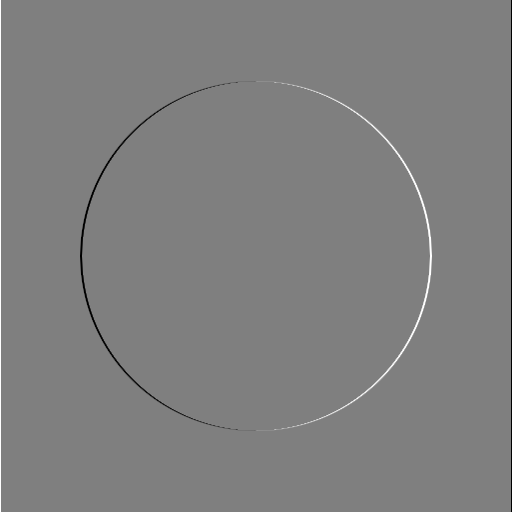
\includegraphics[width=\textwidth]{contenu/resources/images/r2_disk}
        \caption{Première partie impaire}
    \end{subfigure}
    \hfill
    \begin{subfigure}[b]{.3\textwidth}
        
\includegraphics[width=\textwidth]{contenu/resources/images/r1_disk}
        \caption{Seconde partie impaire}
    \end{subfigure}
    \caption[Visualisation du signal monogène pour un disque]{Visualisation du signal monogène pour un disque : le signal original $f$ (gauche) et ses parties impaires $f_{o1}$ (milieu) et  $f_{o2}$ (droite), affichées avec une échelle de couleurs encodant la valeur, de -1 (noir) à +1 (blanc).}
    \label{fig:monogenic-signal-disk}
\end{figure}

Le signal monogène est alors exprimé comme un vecteur à trois composantes, une paire et deux impaires :

\begin{equation}
    f_m(\mathbf{x}) =
    \left[
        \begin{array}{c}
        f_e(\mathbf{x}) \\
        f_{o1}(\mathbf{x}) \\
        f_{o2}(\mathbf{x})
        \end{array}
    \right],
\end{equation}

où $f_e$ est le signal original, indexé par un $e$ pour souligner qu'il représente la partie paire du signal monogène. Une représentation d'un signal et de ses parties impaires est montrée à la figure~\ref{fig:monogenic-signal-disk}. Dans la figure, les parties impaires détectent des changements verticaux et horizontaux dans le signal. La détection des changements est due au fait que la transformée de Riesz présente une ressemblance et une connexion au gradient (l'équation~\ref{eq:2.20} rappelle fortement la définition du gradient, à un facteur près). La transformée de Hilbert présente d'ailleurs aussi une connexion au gradient en 1D. La relation entre les transformées étudiées et le gradient n'est pas le sujet de cette étude et n'est pas explorée plus en profondeur. La personne intéressée se référera à Unser et al.\cite{unser_multiresolution_2009} pour plus de détails.

\bigskip

Il est aussi commun de se représenter le signal monogène comme un vecteur de deux composantes seulement, une paire et une impaire. La composante impaire est alors une combinaison des deux parties impaires présentées ici. Cette représentation est plus compacte, au détriment de la perte d'information sur l'orientation. Elle sera parfois utilisée dans la suite de ce travail :

\begin{equation}
    f_o(\mathbf{x}) = \sqrt{f_{o1}(\mathbf{x})^2 + f_{o2}(\mathbf{x})^2}.
\end{equation}

La transformée de Riesz peut s'exprimer directement dans le domaine spatial. Comme la transformée de Hilbert, la représentation spatiale de la transformée de Riesz est un objet mathématique compliqué, une intégrale singulière :

\begin{equation}
    R_if(x) = c_d \lim_{\epsilon \to 0}\int_{\mathbb{R}^d\setminus B_\epsilon(x)}\frac{(x_i-t_i)f(t)}{|x-t|^{d+1}}\,dt,
    \label{eq:riesz-transform-spatial}
\end{equation}

pour $i\in\llbracket 0, d\rrbracket$ avec $d$ la dimension. $c_d$ est une constante de normalisation dimensionnelle :

\begin{equation}
    c_d = \frac1{\pi\omega_{d-1}} = \frac{\Gamma((d+1)/2)}{\pi^{(d+1)/2}},
\end{equation}

avec $\omega_{d-1}$ le volume de la $(d-1)$-sphère unité. Au vue de la complexité de calcul et de manipulation de cette expression, la formulation fréquentielle est utilisée dans la suite du travail.

\subsubsection{Amplitude, phase et orientation locales}

Avec le signal monogène, le concept d'informations locales est maintenant dérivable pour des images. En 1D, les deux parties du signal analytiques sont représentées en coordonnées polaires avec l'amplitude et la phase. En 2D il y a trois parties à représenter. Les coordonnées sphériques sont donc utilisées. En coordonnées sphériques trois composantes sont définies : le rayon, l'angle d'élévation et l'azimut, comme montré en figure~\ref{fig:spherical-representation}.

\bigskip

\begin{figure}
    \centering
    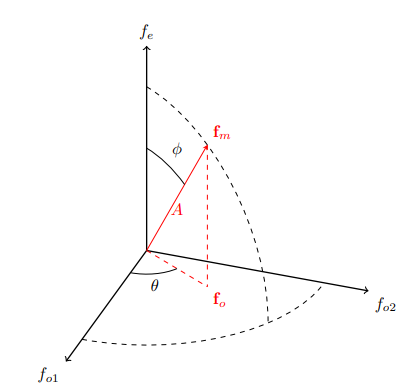
\includegraphics[width=.45\textwidth]{contenu/resources/images/spherical_representation}
    \caption[Représentation du signal monogène en coordonnées sphériques]{Représentation du signal monogène $f_m$ (rouge) en coordonnées sphériques, où les axes sont les différentes parties du signal. Le rayon représente l'amplitude locale, l'angle d'élévation $\phi$ la phase locale et l'azimut $\theta$ l'orientation locale.}
    \label{fig:spherical-representation}
\end{figure}

L'amplitude locale $A$ représente, comme en 1D, le rayon de la représentation :

\begin{align}
    A(\mathbf{x}) &= \sqrt{f_e(\mathbf{x})^2 + f_{o1}(\mathbf{x})^2 + f_{o2}(\mathbf{x})^2} \\
    &= \sqrt{f_e(\mathbf{x})^2 + f_o(\mathbf{x})^2}.
\end{align}

La phase locale $\phi$ mesure l'angle entre la partie paire $f_e$ et la partie impaire combinée $f_o$. La phase représente ainsi l'angle d'élévation de la représentation :

\begin{equation}
    \phi(\mathbf{x}) = \arctan\left(\frac{f_o(\mathbf{x})}{f_e(\mathbf{x})}\right).
\end{equation}

Enfin l'orientation locale $\theta$ complète la représentation en donnant l'angle d'azimut. L'orientation locale indique la direction dominante dans l'image à cet endroit, exprimée comme l'orientation de la partie impaire $f_o$ :

\begin{equation}
    \theta(\mathbf{x}) = \arctan\left(\frac{f_{o2}(\mathbf{x})}{f_{o1}(\mathbf{x})}\right).
\end{equation}

La figure~\ref{fig:monogenic-local-representation} montre un exemple de représentation locale pour une image, avec l'amplitude, la phase et l'orientation locales.

\bigskip

\begin{figure}
    \centering
    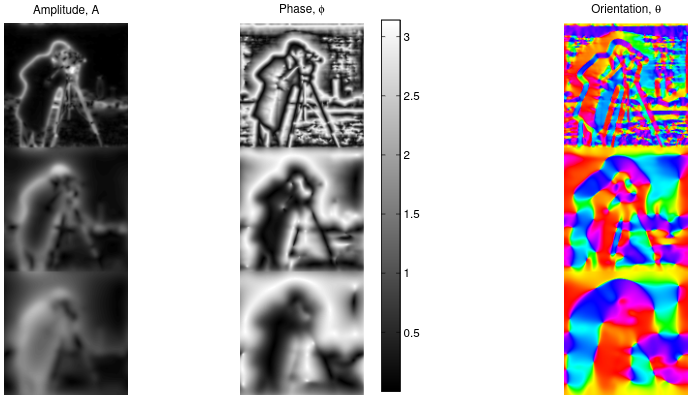
\includegraphics[width=\textwidth]{contenu/resources/images/local_information_monogenic}
    \caption[Représentation locale du signal monogène]{Représentation locale du signal monogène pour une image, avec l'amplitude (gauche), la phase (milieu) et l'orientation (droite) locales. Image par Bridge~\cite{bridge_introduction_2018}.}
    \label{fig:monogenic-local-representation}
\end{figure}

Le changement de représentation est réversible. Le signal monogène peut être reconstruit à partir de ses informations locales :

\begin{equation}
    f_m(\mathbf{x}) = A(\mathbf{x})\left[
        \begin{array}{c}
        \cos(\phi(\mathbf{x})) \\
        \sin(\phi(\mathbf{x}))\cos(\theta(\mathbf{x})) \\
        \sin(\phi(\mathbf{x}))\sin(\theta(\mathbf{x}))
        \end{array}
    \right].
\end{equation}

Notamment, l'image originale s'exprime simplement par $f(\mathbf{x}) = A(\mathbf{x})\cos(\phi(\mathbf{x}))$. Cette formule est utilisée plus tard dans ce travail pour reconstruire les images après modification de leurs informations locales.

\bigskip

Comme pour le signal analytique en 1D, des filtres peuvent être utilisés pour sélectionner un niveau d'échelle à analyser. Sélectionner un niveau d'échelle permet ici encore d'extraire de l'information sur certains niveaux de structure en particulier. Les filtres log-Gabor peuvent être étendus en 2D et utilisés pour sélectionner certaines parties du signal~\ref{fig:2D-log-gabor}.

\bigskip

\begin{figure}
    \centering
    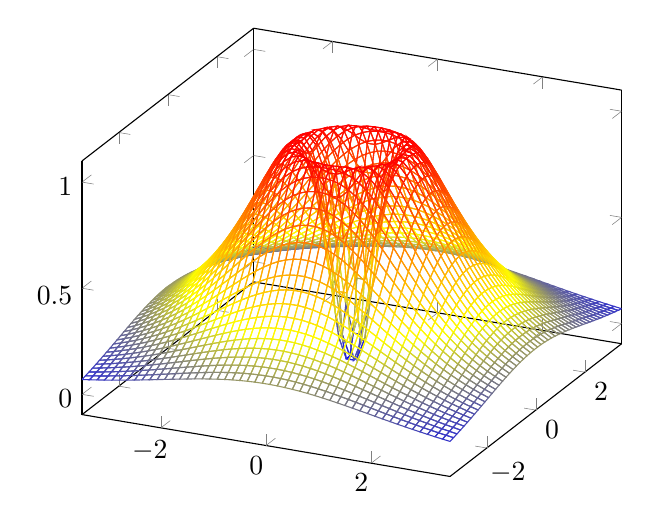
\begin{tikzpicture}
    \begin{axis}[
        colormap/hot,
%        xtick={-.5, 0, .5},
%        ytick={-.5, 0, .5},
%        ztick={-1, 0, 1}
    ]
        \addplot3[
        mesh,
        samples=50,
        domain=-3.5:3.5,
        ]
        {exp(-(ln(sqrt(x^2+y^2))^2)/(2*ln(.5)^2))};
    \end{axis}
    \end{tikzpicture}

    \caption[Filtre log-Gabor en 2D]{Représentation en domaine fréquentiel d'un filtre log-Gabor. Comme en 1D, le filtre sélectionne une bande de fréquence centrée autour d'une fréquence centrale $\omega_0$ et de largeur de bande $\sigma_0$.}
    \label{fig:2D-log-gabor}
\end{figure}

Les parties paires et impaires du signal sont calculées en sélectionnant plusieurs échelles différentes. Les représentations locales créées à chaque niveau d'échelle mettent en valeur les différents niveaux de structure présents dans l'image. La figure~\ref{fig:cameraman-monogenic} montre une image et son signal monogène, calculé sur plusieurs niveaux d'échelle.

\begin{figure}
    \centering
    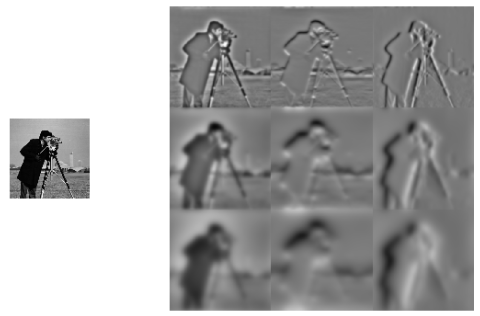
\includegraphics[width=.75\textwidth]{resources/images/cameraman_monogenic}
    \caption[Signal monogène calculé pour plusieurs niveaux d'échelle]{Image originale (gauche) et son signal monogène (droite), calculé sur plusieurs niveaux d'échelle. Dans l'image de droite : en colonne les différentes parties, paire $f_e$ (gauche), impaire 1 $f_{o1}$ (milieu) et impaire 2 $f_{o2}$ (droite). En ligne les longueurs d'onde centrale $\lambda_0 = 2\pi/\omega_0$, caractéristiques de l'échelle de structure détectée : $\lambda_0 = 20$~pixels (haut), $\lambda_0 = 60$~pixels (milieu), $\lambda_0 = 100$~pixels (bas). Pour référence, la taille de l'image originale est 256 $\times$ 256 pixels. Image par Bridge~\cite{bridge_introduction_2018}.}
    \label{fig:cameraman-monogenic}
\end{figure}

\bigskip

Le cadre de travail pour le restant du manuscript, le signal monogène, a été introduit. Le cadre choisi pour travailler à différents niveaux de structure va maintenant être discuté. Bridge présente dans son article~\cite{bridge_introduction_2018} un cadre de travail utilisant les filtres log-Gabor. Les filtres log-Gabor 2D possèdent une expression complexe dans le domaine spatial. Pour les travaux présentés, une autre méthode de représentation est utilisée : la pyramide de Riesz. Les calculs nécessaires à la création et manipulation de la pyramide de Riesz sont plus élémentaires que ceux des filtres log-Gabor. Le choix de la simplicité pour les calculs permet de concentrer les efforts de recherche sur l'analyse de textures. La section qui suit introduit la pyramide de Riesz et montre comment elle peut être utilisée pour l'analyse de textures.

\section{Pyramide de Riesz}

L'idée de travailler en considérant plusieurs niveaux d'échelle est introduite par Burt et Adelson~\cite{burt_laplacian_1983} pour la compression d'images. La méthode de la pyramide d'image mise au point par Burt et Adelson est une méthode de représentation multi-échelle utilisée dans les domaines de la vision par ordinateur et du traitement d'image pour la résolution de nombreux problèmes comme la détection de motifs. Une pyramide d'images remplit la même fonction qu'une banque de filtres, comme les filtres log-Gabor utilisés par Bridge. Une image est décomposée en sélectionnant successivement différentes bandes de fréquences. De l'information localisée en fréquence est ainsi extraite.

\bigskip

La pyramide d'image est ensuite étendue par Simoncelli et al.~\cite{simoncelli_shiftable_1992}. La pyramide de Simoncelli et al., dite orientable, a des propriétés d'invariance par rotation, translation et mise à l'échelle. Les propriétés d'invariance de la pyramide orientable sont une amélioration par rapport aux modèles précédent. La pyramide orientable sert de base à la pyramide de Riesz utilisée dans ces travaux. Wadhwa et al.~\cite{wadhwa_phase_based_2013} mettent au point la pyramide de Riesz pour étudier les micro-mouvements dans des vidéos. La pyramide utilisée dans les travaux présentés est fortement inspirée de Wadhwa et al. La construction de la pyramide, plus détaillée dans les paragraphes qui suivent, s'organise comme suit. Dans un premier temps les pyramides gaussienne puis laplacienne sont formées. La pyramide laplacienne offre une méthode de reconstruction de l'image. La transformée de Riesz est ensuite appliquée à tous les étages de la pyramide pour obtenir le signal monogène de chaque niveau. Les informations locales des différents niveaux sont enfin extraites pour analyser les différents niveaux de structure. La pyramide de Riesz est un outil d'analyse qui sera par la suite utilisée pour l'analyse et la synthèse de textures.

\subsection{Pyramide gaussienne}

Il existe deux types principaux de pyramide, passe-bas et passe-bande. Pour créer une pyramide passe-bas, aussi dite \og gaussienne \fg, deux étapes sont répétées itérativement :

\bigskip

\begin{itemize}
    \item une étape de \og lissage \fg (ou filtrage) de l'image, qui consiste à appliquer un filtre passe-bas à l'image, afin de supprimer les hautes fréquences. Une image lissée est formée, où les détails fins ont été supprimés ;
    \item une étape de \og sous-échantillonnage \fg, qui consiste à réduire la taille de l'image en gardant un pixel sur deux dans chaque direction. L'image obtenue a la moitié de la taille de l'image originale.
\end{itemize}

\bigskip

Les deux étapes sont répétées sur l'étage nouvellement créé, et ce jusqu'à atteindre la profondeur désirée. Le résultat est une collection d'images de plus en plus petites et de moins en moins raffinées (en termes de résolution). Un exemple est donné en figure~\ref{fig:gaussian-pyramid}. La collection d'images peut être représentée graphiquement comme une pyramide en superposant les étages du plus grand au plus petit, comme montré à la figure~\ref{fig:pyramid-gauss}.

\begin{figure}[h]
    \centering

    \begin{subfigure}{.3\textwidth}
        \centering
        
\includegraphics[width=\textwidth]{contenu/resources/images/gauss_0}
        \caption{Image originale}
    \end{subfigure}
    \hfill
    \begin{subfigure}{.3\textwidth}
        \centering
        
\includegraphics[width=\textwidth]{contenu/resources/images/gauss_3}
        \caption{Étage 3}
    \end{subfigure}
    \hfill
    \begin{subfigure}{.3\textwidth}
        \centering
        
\includegraphics[width=\textwidth]{contenu/resources/images/gauss_5}
        \caption{Étage 5}
    \end{subfigure}
%    \hfill
%    \begin{subfigure}{.22\textwidth}
%        \centering
%        
\includegraphics[width=\textwidth]{contenu/resources/images/gauss_3}
%        \caption{Étage 3}
%    \end{subfigure}

    \caption[Étages de la pyramide de Gauss]{Étages de la pyramide de Gauss. De gauche à droite, les étages sont de plus en plus petits.}
    \label{fig:gaussian-pyramid}
\end{figure}

Différents noyaux de lissage ont été proposés dans la littérature. La famille des noyaux binomiaux par exemple est fréquemment utilisée. L'implémentation proposée dans ce travail utilise les noyaux binomiaux, qui s'expriment à l'aide des coefficients binomiaux :

\begin{equation}
    k = \frac{1}{256}\left[
        \begin{array}{ccccccc}
            1 & 4 & 6 & 4 & 1 \\
            4 & 16 & 24 & 16 & 4 \\
            6 & 24 & 36 & 24 & 6 \\
            4 & 16 & 24 & 16 & 4 \\
            1 & 4 & 6 & 4 & 1
        \end{array}
    \right],
\end{equation}

Il est intéressant de constater que les pyramides gaussiennes sont notamment utilisées dans la synthèse de texture. En effet les MIP maps employées pour remédier au sous-échantillonnage sont un pré-calcul des textures à différents niveaux de résolution ; ce sont des pyramides gaussiennes.

\begin{figure}
    \centering
    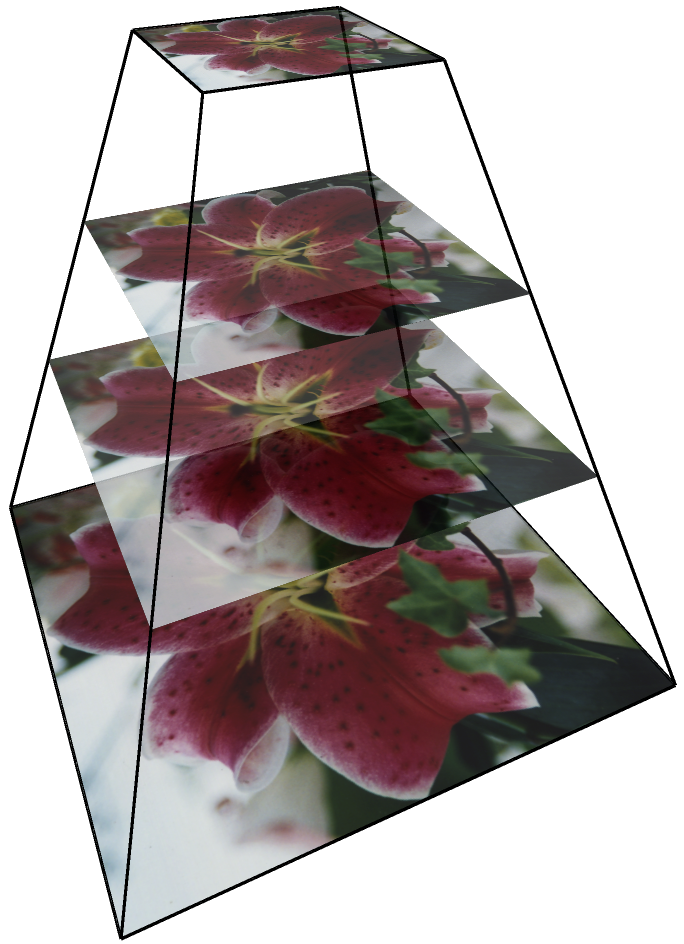
\includegraphics[width=.25\textwidth]{contenu/resources/images/image_pyramid_placeholder}
    \caption[Représentation pyramidale des étages de la pyramide de Gauss]{Représentation en pyramide des étages de la pyramide de Gauss. Crédit à \textit{Isnomore} pour l'image}
    \label{fig:pyramid-gauss}
\end{figure}

\subsection{Pyramide laplacienne}

La \og pyramide laplacienne \fg est une autre forme de pyramide qui correspond à un type passe-bande. Comme l'expliquent Burt et Adelson~\cite{burt_laplacian_1983}, les texels voisins dans une image sont souvent hautement corrélés. Encoder une image en termes de valeur de pixels cause une perte d'efficacité à cause de la redondance d'information. Il est possible d'encoder une image plus efficacement, c'est-à-dire avec moins de bits. La pyramide laplacienne est une représentation qui décorelle les texels voisins et qui répond donc à cette problématique.

\subsubsection{Construction de la pyramide}

Plutôt que d'encoder la valeur même de chaque pixel, une prédiction est faite sur la valeur que chaque pixel devrait avoir. C'est l'erreur de prédiction qui est alors encodée. La valeur prédite de chaque pixel est obtenue en calculant une moyenne pondérée locale centrée autour du pixel. Dans un premier temps, une image lissée est créée par convolution. La convolution par filtre correspond au calcul de la moyenne pondérée. L'image lissée représente les corrélations locales entre les texels au niveau d'échelle correspondant au filtre choisi. L'image lissée comporte les éléments redondants à encoder plus efficacement. Pour améliorer l'encodage, l'image lissée est soustraire à l'image originale. L'image obtenue exprime l'erreur de prédiction pour chaque texel. La relation suivante illustre le procédé :

\begin{equation}
    L = I - k * I,
\end{equation}

avec $I$ l'image originale, $L$ l'image d'erreur de prédiction et $k$ le filtre de moyenne pondérée. Pour la compression d'images, l'intérêt se trouve dans cette ré-écriture. Les pixels de $L$ sont décorrélés et de faible valeur, donc encodables avec peu de bits. $k*I$ est une image lissée, qui peut être sous-échantillonnée pour obtenir une image de moitié de taille. L'image est représentée par $L$ et $k*I$ uniquement et cette représentation est plus compacte que l'image originale.

\bigskip

Le processus est répétable itérativement, en appliquant à chaque fois le même filtre à l'image lissée de résolution inférieure. La figure~\ref{fig:gauss-laplace-pyramid} illustre le processus itératif de construction de la pyramide laplacienne. Seules les images d'erreur, dont la taille est divisée par 4 à chaque fois, sont enregistrées. La dernière image lissée, est de taille $N/2^{2d}$, avec $N$ la taille de l'image initiale et $d$ la profondeur désirée. Encore une fois, la collection d'images est représentable comme une pyramide, en superposant les images de la plus grande à la plus petite.

\bigskip

Le filtre de lissage utilisé est un filtre passe-bas, qui moyenne localement l'image. Le même genre de filtre passe-bas est utilisé pour créer une pyramide gaussienne. En fait, une pyramide gaussienne est souvent utilisée pour construire une pyramide laplacienne. La pyramide gaussienne représente toutes les images lissées nécessaires à la construction de la pyramide laplacienne. La pyramide gaussienne est calculée, puis à chaque étage est soustrait l'étage de résolution inférieure. Les images d'erreur de prédiction sont obtenus à partir de la pyramide gaussienne.

\bigskip

Pour soustraire une image lissée à son image de taille originale, une étape d'expansion est nécessaire. Une méthode communément utilisée pour l'expansion consiste à doubler la taille de l'image, en insérant des zéros entre chaque pixel, puis à appliquer un filtre passe-bas à l'image résultante. L'image résultante est une image de taille double qui est une approximation de l'image lissée. Cette image est alors soustraite à l'image originale pour obtenir l'image d'erreur de prédiction.

\begin{figure}
    \centering
    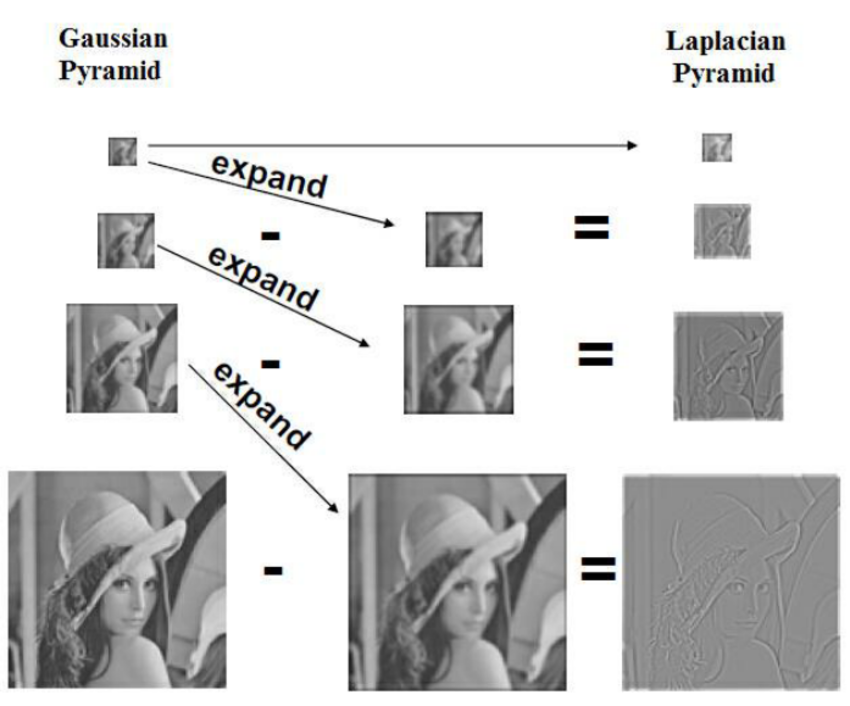
\includegraphics[width=.75\textwidth]{contenu/resources/images/gauss_laplace_pyramid}
    \caption[Relation entre pyramide gaussienne et laplacienne]{Processus de création de la pyramide laplacienne à partir de ma pyramide gaussienne. Crédit à \textit{Jebamalar et Sutha}~\cite{jebamalar_design_2014} pour l'image.}
    \label{fig:gauss-laplace-pyramid}
\end{figure}

\subsubsection{Reconstruction de l'image}

L'image décomposée en pyramide laplacienne est stockée en enregistrant les images d'erreur de prédiction et l'image lissée de plus basse résolution. Pour reconstruire l'image originale, un processus itératif est utilisé. Le résidu basse fréquences est additionné à la dernière image d'erreur pour former une image lissée de résolution supérieure. Le processus est répété en additionnant à chaque fois l'image lissée obtenue à l'image d'erreur suivante, jusqu'à obtenir l'image originale.

\bigskip

Avec une pyramide gaussienne, les images lissées sont de taille différente (divisée par 4 à chaque fois). Deux images doivent avoir la même taille pour pouvoir être soustraites l'une à l'autre. Pour s'assurer que les images ont la même taille, les images lissées sont étendues à chaque étape. La même opération d'expansion que celle de la création de la pyramide est utilisée pour étendre les images. Le processus de reconstruction est montré à l'image~\ref{fig:laplace-reconstruction}.

\begin{figure}
    \centering
    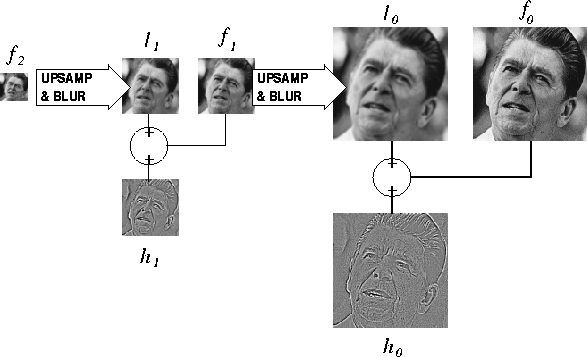
\includegraphics[width=.85\textwidth]{contenu/resources/images/laplacian_pyramid_reconstruction}
    \caption[Reconstruction d'une image à partir de sa pyramide laplacienne]{Reconstruction d'une image à partir de sa pyramide laplacienne. $f_i$ les images de la pyramide gaussienne, $h_i$ celles de la pyramide laplacienne, et $l_i$ les images lissées étendues. Image de \href{https://web.archive.org/web/20230203082428/http://sepwww.stanford.edu/data/media/public/sep/morgan/texturematch/paper_html/node3.html}{Stanford Exploration Project}.}
    \label{fig:laplace-reconstruction}
\end{figure}

\subsection{Pyramide de Riesz}

La \og pyramide de Riesz \fg est une extension de la pyramide laplacienne. C'est le cadre permet l'étude du signal monogène d'une image à différents niveaux d'échelle. La pyramide de Riesz est construite en appliquant la transformée de Riesz à chaque étage de la pyramide laplacienne. La pyramide de Riesz est illustrée à la figure~\ref{fig:riesz-pyramid-cameraman}. Les informations locales sont ensuite calculées pour chaque étage de la pyramide. Les informations locales des différents niveaux sont mis en relation dans la suite des travaux afin plus d'information sur l'image, comme expliqué dans le chapitre implémentations~\ref{chap:chapitre2}.

\bigskip

\begin{figure}
    \centering
    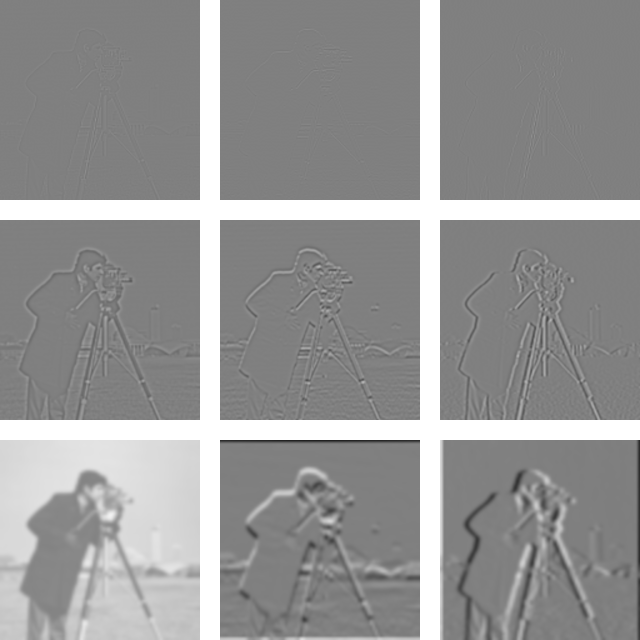
\includegraphics[width=.65\textwidth]{contenu/resources/images/riesz_pyramid_cameraman}
    \caption[Pyramide de Riesz]{Différents étages de la pyramide de Riesz, calculée avec la transformée de Riesz approximée. En colonne, les différentes composantes : l'image originale de la pyramide laplacienne (gauche), puis les deux composantes de Riesz (milieu et droite). En ligne, les différents étages de la pyramide : étage 0 (haut), étage 2 (milieu) et étage 3, le dernier (bas).}
    \label{fig:riesz-pyramid-cameraman}
\end{figure}

Pour des raisons de vitesse de calcul et de simplicité d'implémentation, la vraie transformée de Riesz n'est pas utilisée dans ce travail. La transformée de Riesz nécessite une transformation de l'image dans le domaine de Fourier ou le calcul d'une intégrale singulière (voir l'équation~\ref{eq:riesz-transform-spatial}), deux méthodes qui sont complexes à opérationnaliser. À la place, l'approximation proposée par Wadhwa et al.~\cite{wadhwa_riesz_2014} est utilisée. L'approximation de Wadhwa et al. se calcule directement dans le domaine spatial en utilisant les filtres à réponse impulsionnelle finie $[-0.5, 0, 0.5]$ et $[-0.5, 0, 0.5]^T$, dont les réponses en fréquence sont :

\begin{equation}
    -i\sin(\omega_x) \quad \text{et} \quad -i\sin(\omega_y).
\end{equation}

Cette approximation donne de bons résultats ici, car les filtres ont une réponse équivalente à celle de la transformée de Riesz aux alentours de $\frac\pi2$, où se concentre la majorité de l'énergie des images dans la pyramide laplacienne~\cite{wadhwa_riesz_2014}. En $0$, il y a une différence notable entre la réponse des filtres et la réponse de la transformée de Riesz. Cependant, le contenu fréquentiel est faible en $0$ puisque, par construction, le contenu basse fréquences est supprimé dans la pyramide laplacienne. L'erreur due à la différence en $0$ est donc faible aussi. La figure~\ref{fig:riesz-approximation} montre une comparaison entre l'application de la transformée de Riesz et de son approximation. Les informations locales pour chaque étage, amplitude, phase et orientation, sont ensuite calculées comme expliqué dans la section précédente. La figure~\ref{fig:riesz-pyramid-local} présente les informations locales obtenues avec la pyramide de Riesz.

\bigskip

\begin{figure}[h]
    \centering
    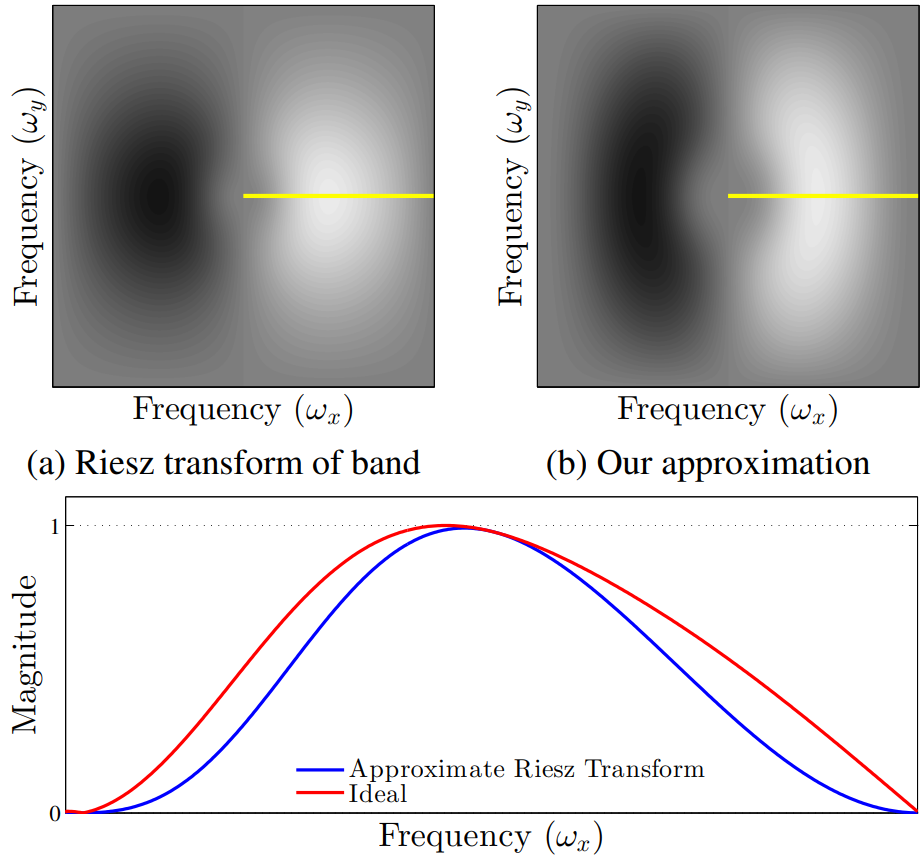
\includegraphics[width=.65\textwidth]{contenu/resources/images/riesz_approximation}
    \caption[Approximation de la transformée de Riesz]{Comparaison de l'application de la transformée de Riesz (gauche) et de son approximation (droite) pour un niveau de pyramide. Les tranches horizontales en jaune sur les images (a) et (b) sont représentées dans le diagramme en (c). Image par Wadhwa et al.~\cite{wadhwa_riesz_2014}.}
    \label{fig:riesz-approximation}
\end{figure}

\begin{figure}[hp]
    \centering
    \includegraphics[width=.90\textwidth]{contenu/resources/images/riesz_pyramid_pasta}
    \caption[Informations locales de la pyramide de Riesz]{Informations locales de la pyramide de Riesz. En colonne, les différentes composantes : en colonne, les différentes informations locales : amplitude (gauche), phase (milieu) et orientation (droite). En ligne les différentes étages de la pyramide, du premier (haut) au dernier (bas).}
    \label{fig:riesz-pyramid-local}
\end{figure}

Avec cette implémentation de la pyramide de Riesz, le cadre d'étude multi-résolutionnel local a été défini. La prochaine partie décrit comment le cadre multi-résolutionnel local est utilisé afin d'extraire de l'information d'une texture.

\section{Congruence de phases}

Le modèle de l'énergie locale est un modèle de détection de caractéristiques saillantes dans une image. Introduit par Morrone et al~\cite{morrone_mach_1986, morrone_feature_1987},il explique la présence de points saillants, tels que des bords et des coins, par l'alignement des phases locales de l'image. Le modèle d'énergie locale est basé sur l'observation que les bords et les coins sont des structures résultant de la superposition de sinusoïdes en phase les unes avec les autres. Contrairement aux autres méthodes de détection de caractéristiques, comme celles de Sobel ou Canny, le modèle de Morrone et al. est insensible aux variations de luminosité et de grossissement. Les méthodes par gradient utilisent en effet un seuillage pour déterminer les bords, qui dépend de la luminosité et du niveau de zoom de l'image. À l'inverse, le modèle de l'énergie locale permet le calcul de la \og congruence de phases \fg (PC), une grandeur à valeurs dans $[0, 1]$ mesurant uniformément la présence d'éléments caractéristiques dans une image et la proximité d'un texel à un élément caractéristique. La congruence de phases est le sujet de la partie qui suit.

\bigskip

La formulation initiale de la PC utilise les coefficients de la série de Fourier du signal. Cependant, cette formulation comporte trois problèmes : elle est difficile à calculer et manipuler, elle ne permet pas une bonne localisation de l'information (le même problème qui pousse à utiliser un cadre de travail multi-résolutionnel pour l'étude du signal monogène), et elle ne prend pas en compte la répartition des fréquences. Ces problèmes et leur solution sont expliqués dans un premier temps en 1D, puis en 2D.

\subsubsection{Énergie locale}

Venkatesh et Owens~\cite{venkatesh_energy_1989} montrent qu'il existe une relation directe entre la PC et l'énergie locale. Ils mettent ainsi en lumière une expression simplifiée de la PC :

\begin{equation}
    PC(x) = \frac{E(x)}{\sum_{n=0}^{+\infty} D_n},
\end{equation}

avec $E(x) = \sqrt{f^2(x) + f_h^2(x)}$ l'énergie locale et $D_n$ les coefficients d'amplitude de la série de Fourier du signal :

\begin{equation}
    f(x) = \sum_{n=0}^{+\infty} D_n\cos(n\omega x + \phi_n).
    \label{eq:phase-congruence-energy}
\end{equation}


\subsubsection{Contexte multi-résolutionnel}

Pour obtenir de l'information localisée en termes de fréquence et sélectionner successivement différents niveaux d'échelle, Kovesi utilise des ondelettes sous forme de banque de filtres passe-bande. Les filtres passe-bande utilisés sont des filtres de Gabor, très similaires à ceux présentés dans la section introduisant le signal monogène~\ref{subsubsec:echelle}. En faisant la convolution du signal par ces filtres, il obtient de l'information localisée à la fois spatialement et fréquentiellement :

\begin{equation}
    A_n(x) = \sqrt{(f(x)*M^e_n)^2 + (f(x)*M^o_n)^2},
    \label{eq:local-scale-amplitude}
\end{equation}

et

\begin{equation}
    \phi_n(x) = \arctan\left(\frac{f(x)*M^o_n}{f(x)*M^e_n}\right),
\end{equation}

avec $M^e_n$ et $M^o_n$ les filtres passe-bande, paire et impaire, au niveau d'échelle $n$. À noter que le $n$ dans l'équation~\ref{eq:local-scale-amplitude}, entre 1 et $N$ (le nombre de nivaux d'échelle considéré), désigne le niveau d'échelle fréquentiel. Il est différent de celui dans l'équation de la série de Fourier~\ref{eq:phase-congruence-energy} qui, lui, représente les différentes sinusoïdes qui forment le signal. L'intérêt de la PC est exposé à la figure~\ref{fig:phase-congruence-scalogram} qui représente les scalogrammes de phase et d'amplitude d'un signal 1D. Les points saillants sont ceux où la phase est alignée à travers tous les niveaux d'échelle.

\bigskip

\begin{figure}
    \centering
    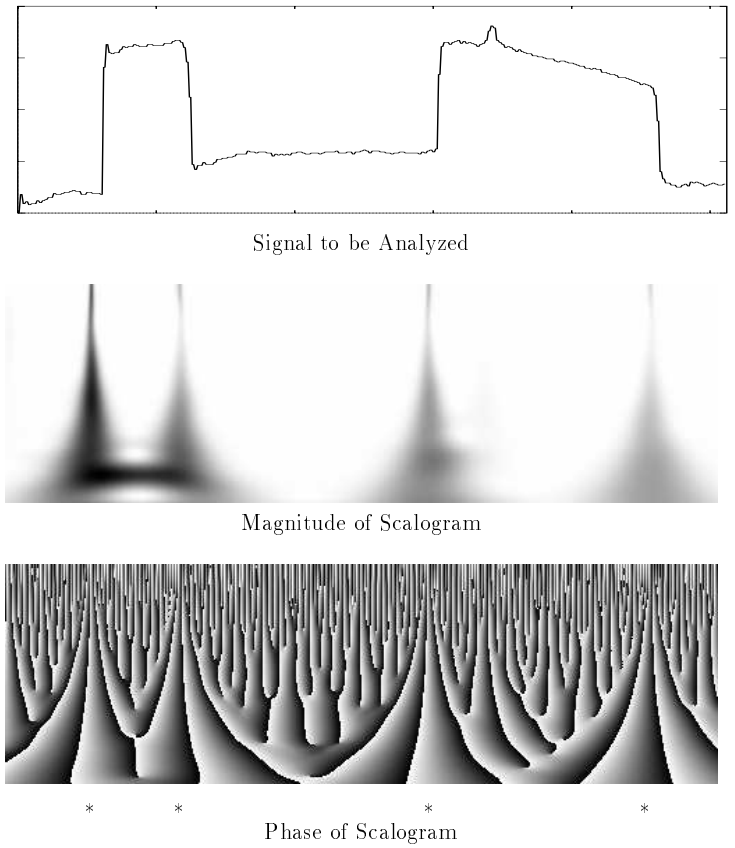
\includegraphics[width=.85\textwidth]{contenu/resources/images/phase_congruence_scalogram}
    \caption[Scalogramme d'un signal mettant en évidence des points caractéristiques du signal]{Signal 1D et ses scalogrammes de phase et d'amplitude. L'abscisse des scalogrammes sont les mêmes que celui du signal, et les ordonnées représentent à la fréquence en échelle logarithmique (valeurs croissantes de bas en haut). Les astérisques marquent les transitions abruptes dans le signal et correspondent aux instants où la phase est alignée à travers tous les niveaux d'échelle. Les astérisques sont des points où la congruence de phases est élevée. Image par Kovesi~\cite{kovesi_image_1995}.}
    \label{fig:phase-congruence-scalogram}
\end{figure}

Une nouvelle expression de la PC qui prend en compte la localisation fréquentielle est dérivée avec les composantes filtrées à différents niveaux d'échelle du signal :

\begin{equation}
    PC(x) = \frac{E(x)}{\sum_{n=1}^{N} A_n(x)} = \frac{\sqrt{F^2(x)+F_H^2(x)}}{\epsilon + \sum_{n=1}^{N}},
\end{equation}

où $F$ et $F_H$ sont une reconstruction du signal et de sa transformée de Hilbert respectivement. Les reconstructions sont obtenues à partir des composantes filtrées :

\begin{align}
    F(x) &= \sum_{n=1}^{N} f(x)*M_n^e, \,\text{et}\\
    F_H(x) &= \sum_{n=1}^{N} f(x)*M{_n^o}.
\end{align}

$\sum_{n=1}^{N} A_n(x)$ indique ici la somme des amplitudes locales à tous les niveaux d'échelle :

\begin{equation}
    \sum_{n=1}^{N} A_n(x) = \sum_{n=1}^{N} \sqrt{(f(x)*M^e_n)^2 + (f(x)*M^o_n)^2}
\end{equation}

avec $\epsilon$ une petite constante positive qui assure la stabilité numérique de l'expression quand la somme des amplitudes est très petite. Dans l'implémentation du calcul de la PC, $\epsilon = 0.01$ est utilisé.

\bigskip

Pour pouvoir reconstruire le signal et sa transformée de Hilbert, le choix des filtres de la transformée en ondelettes est important. Les filtres doivent être choisis de sorte que leur fonction de transfert se superposent lorsqu'additionnées et recouvrent l'entièreté du spectre du signal, comme montré dans la figure~\ref{fig:wavelet-spectrum-coverage}.

\begin{figure}
           \centering
           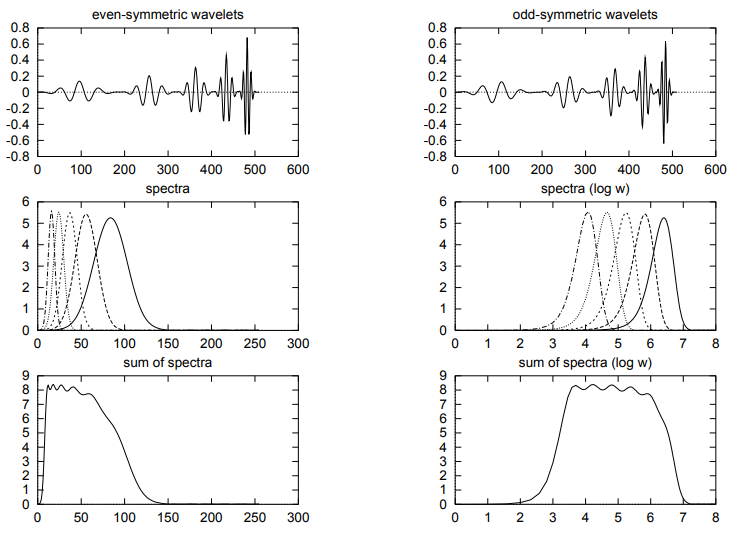
\includegraphics[width=.60\textwidth]{contenu/resources/images/wavelet_spectrum_coverage}
           \caption[Choix des ondelettes pour recouvrir le spectre et permettre la reconstruction du signal]{Banque d'ondelettes choisie de sorte à recouvrir une large couverture du spectre. Les différents diagrammes représentent les ondelettes (haut) et leur fonction de transfert (milieu), ainsi que la fonction de transfert de la somme des ondelettes (bas). Image par Kovesi~\cite{kovesi_image_1995}.}
           \label{fig:wavelet-spectrum-coverage}
\end{figure}

\subsubsection{Répartition des fréquences}

La PC mesure l'alignement des phases à différents niveaux de fréquence. Afin que la PC soit un indicateur significatif, il faut qu'une large bande de fréquences soit couverte. Lorsque le signal a une réponse en fréquence restreinte, dans le cas d'un signal simple ou lissé par exemple, la bande de fréquence couverte est étroite. La PC prend alors des valeurs trop grandes sur des plages trop larges du signal, comme montré dans la figure~\ref{fig:phase-congruency-spread}. La qualité de détection de bords diminue puisque la PC est haute sur de larges régions.

\bigskip

\begin{figure}
    \centering
    \begin{subfigure}{.22\textwidth}
        \centering
        
\includegraphics[width=\textwidth]{contenu/resources/images/disk}
        \caption{Image originale\\}
    \end{subfigure}
%    \hfill
    \begin{subfigure}{.22\textwidth}
        \centering
        
\includegraphics[width=\textwidth]{contenu/resources/images/disk_blur}
        \caption{Image lissée}
    \end{subfigure}
    \\
    \begin{subfigure}{.22\textwidth}
        \centering
        
\includegraphics[width=\textwidth]{contenu/resources/images/pc_blur_nospread}
        \caption{Congruence de phases sans pondération}
    \end{subfigure}
%    \hfill
    \begin{subfigure}{.22\textwidth}
        \centering
        
\includegraphics[width=\textwidth]{contenu/resources/images/pc_blur_spread}
        \caption{Congruence de phases avec pondération}
    \end{subfigure}

    \caption[Congruence de phases pour une image lissée par noyau gaussien]{Comparaison de la congruence de phases pour une image lissée par un noyau gaussien, avec et sans pondération par la répartition de la réponse en fréquence.}
    \label{fig:phase-congruency-spread}
\end{figure}

Pour remédier à ce problème, une fonction de pondération est mise au point. La fonction de pondération diminue l'importance des points où la réponse en fréquence est restreinte. La répartition de la réponse en fréquence est mesurée en comparant la plus grande amplitude locale à celles des autres niveaux d'échelle :

\begin{equation}
    s(x) = \frac1N\left(\frac{\sum_{n=1}^{N}A_n(x)}{\epsilon + A_{max}(x)}\right),
\end{equation}

où $A_{max}(x)$ est la plus grande amplitude parmi ces niveaux et $\epsilon$ est encore une petite constante positive qui assure la stabilité numérique de l'expression. Cette mesure de la répartition de la réponse en fréquence est à valeurs entre 0 et 1 et est utilisée pour construire la fonction de pondération avec la fonction sigmoïde :

\begin{equation}
    W(x) = \frac{1}{1 + \exp^{g(c-s(x))}},
\end{equation}

avec $c$ la valeur de coupure en-dessous de laquelle la réponse en fréquence est considérée restreinte et $g$ un paramètre de gain qui contrôle la précision de la coupure. Dans la pratique, les valeurs $c = 0.4$ et $g = 10$ sont utilisées car elles donnent de bons résultats. La fonction de pondération vaut 1 lorsque la réponse en fréquence est uniformément répartie et décroit lorsque la réponse en fréquence est restreinte. La PC est ré-écrite en tenant compte de cette fonction de pondération :

\begin{equation}
    PC(x) = \frac{W(x)E(x)}{\epsilon + \sum_{n=1}^{N} A_n(x)}.
\end{equation}

\subsubsection{Extension à deux dimensions}

Pour étendre la méthode en deux dimensions, Kovesi utilise une banque de filtres de Gabor 2D auxquels il applique une fonction d'étalement gaussienne, perpendiculairement à la direction du filtre. En variant l'orientation des filtres, il s'assure de recouvrir totalement le spectre de l'image. L'expression de la PC s'étend pour prendre en compte toutes les orientations :

\begin{equation}
    PC(\mathbf{x}) = \frac{\sum_{o\in \mathcal{O}} W_o(x)E_o(\mathbf{x})}{\epsilon + \sum_{o \in \mathcal{O}}\sum_{n=1}^{N} A_{no}(\mathbf{x})}
\end{equation},

où $\mathcal{O}$ est l'ensemble des orientations utilisées dans la banque de filtres. Le calcul de la répartition des fréquences $W_o(x)$ doit aussi se faire pour chaque orientation.

\subsubsection{Utilisation du cadre multi-résolutionnel local de Riesz}

Le but du travail présenté est d'appliquer le modèle de la PC pour synthétiser des textures présentant de la structure irrégulière. Cependant, le cadre multi-résolutionnel local de Riesz présenté précédemment nous semble plus intéressant que les banques d'ondelettes de Gabor présentée par Kovesi~\cite{kovesi_image_1995}, car il est plus compact, plus simple à implémenter et donne plus d'informations. Notamment, il donne accès à l'orientation locale en chaque pixel de l'image, information pertinente pour l'analyse de texture. Le modèle de la PC est donc adapté au cadre de travail avec une pyramide de Riesz :

\begin{equation}
    PC(\mathbf{x}) = \frac{W(x)E(\mathbf{x})}{\epsilon + \sum_{n=0}^{d} A_{n}(\mathbf{x})} = \frac{W(x)\sqrt{F^2(\mathbf{x})+R_1^2(\mathbf{x})+R_2^2(\mathbf{x})}}{\epsilon + \sum_{n=0}^{d} \sqrt{f_n^2(\mathbf{x}) + r_{1n}^2(\mathbf{x}) + r_{2n}^2(\mathbf{x})}},
\end{equation}

avec $d$ la profondeur de la pyramide, $f_i, r_{1i}\, \text{et}\, r_{2i}$ les composantes de Riesz de l'étage $i$. $F, R_1$ et $R_2$ sont les reconstructions de l'image originale et des composantes de sa transformée de Riesz, qui se calculent avec les différents étages de la pyramide :

\begin{equation}
    F(\mathbf{x}) = \sum_{n=0}^{d} f_n(\mathbf{x}) \quad \text{et} \quad R_i(\mathbf{x}) = \sum_{n=0}^{d} r_{in}(\mathbf{x})\, \text{pour}\, i \in \{1, 2\}.
\end{equation}

\begin{figure}
    \centering
    \begin{subfigure}{.3\textwidth}
        \centering
        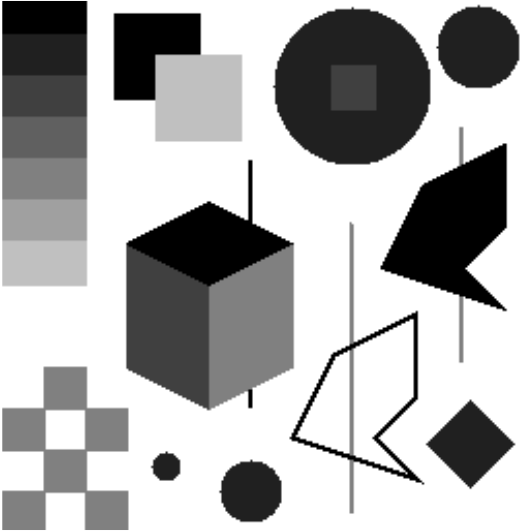
\includegraphics[width=\textwidth]{contenu/resources/images/geometry_shapes}
        \caption{Image originale}
    \end{subfigure}
    \hfill
    \begin{subfigure}{.3\textwidth}
        \centering
        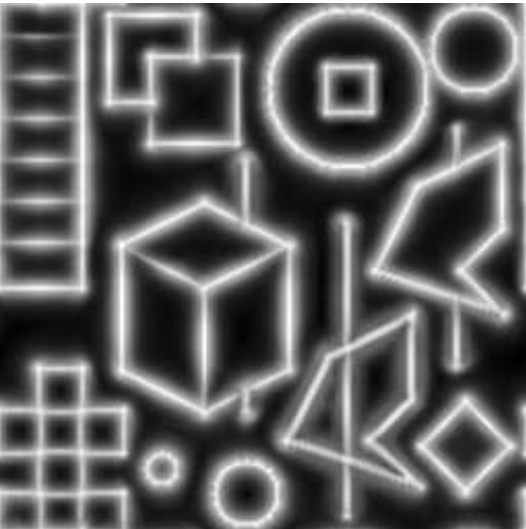
\includegraphics[width=\textwidth]{contenu/resources/images/geometric_shapes_pc_kovesi}
        \caption{Congruence de phases de Kovesi}
    \end{subfigure}
    \hfill
    \begin{subfigure}{.3\textwidth}
        \centering
        
\includegraphics[width=\textwidth]{contenu/resources/images/geometric_shapes_pc_riesz}
        \caption{Congruence de phases de Riesz}
    \end{subfigure}

    \caption[Comparaison de la congruence de phases de Kovesi et de Riesz pour une image de test de formes géométriques]{Comparaison de la congruence de phases de Kovesi et de Riesz pour une image de test de formes géométriques.}
    \label{fig:phase-congruency-riesz}
\end{figure}

\bigskip

Avec cette formulation, une méthode de calcul de la PC a été définie pour le cadre multi-résolutionnel local de Riesz. Une comparaison entre la PC de Kovesi et celle proposée dans ce travail est faite à la figure~\ref{fig:phase-congruency-riesz}. Le chapitre suivant décrit comment la méthode a été implémentée et comment elle est utilisée pour la synthèse de texture.